% =====================================================================
%  Sensor Accuracy Worksheet --- Cadence (ankle freeze-of-gait monitor)
%  ENGF0031 Scenario 2 "Smart Clothing"
%  All quantitative results in this document are computed from real
%  on-body captures and the project's analysis code (no fabricated data).
% =====================================================================
\documentclass[11pt,a4paper]{article}

\usepackage[utf8]{inputenc}
\usepackage[T1]{fontenc}
\usepackage{lmodern}
\usepackage[a4paper,margin=2.3cm]{geometry}
\usepackage{graphicx}
\usepackage{booktabs}
\usepackage{array}
\usepackage{amsmath}
\usepackage{amssymb}
\usepackage{xcolor}
\usepackage{enumitem}
\usepackage{caption}
\usepackage{float}
\usepackage{listings}
\usepackage[most]{tcolorbox}
\usepackage{fancyhdr}
\usepackage{titlesec}
\usepackage[hidelinks]{hyperref}
\usepackage{siunitx}

\graphicspath{{accuracy_figs/}{accuracy_figs/smoketest_out/}}

% ---- palette -------------------------------------------------------
\definecolor{navy}{HTML}{1E2761}
\definecolor{steel}{HTML}{34618E}
\definecolor{brick}{HTML}{C0392B}
\definecolor{ink}{HTML}{222222}
\definecolor{mist}{HTML}{EEF2F8}
\definecolor{rule}{HTML}{C9D3E4}
\definecolor{codebg}{HTML}{F6F8FA}
\definecolor{hlbg}{HTML}{FCEFC7}

% ---- headers -------------------------------------------------------
\pagestyle{fancy}
\fancyhf{}
\renewcommand{\headrulewidth}{0.4pt}
\renewcommand{\footrulewidth}{0pt}
\lhead{\small\textsc{Accuracy Worksheet}}
\rhead{\small Cadence --- Ankle FoG Monitor}
\cfoot{\small\thepage}

% ---- section styling ----------------------------------------------
\titleformat{\section}{\Large\bfseries\color{navy}}{\thesection}{0.6em}{}
\titleformat{\subsection}{\large\bfseries\color{ink}}{\thesubsection}{0.5em}{}
\titlespacing*{\section}{0pt}{1.4em}{0.6em}

% ---- listings ------------------------------------------------------
\lstdefinestyle{cpp}{
  language=C++, backgroundcolor=\color{codebg}, basicstyle=\ttfamily\scriptsize,
  keywordstyle=\color{navy}\bfseries, commentstyle=\color{steel}\itshape,
  stringstyle=\color{brick}, numbers=left, numberstyle=\tiny\color{gray},
  numbersep=8pt, breaklines=true, frame=single, rulecolor=\color{rule},
  showstringspaces=false, tabsize=2, columns=fullflexible, captionpos=b}
\lstdefinestyle{py}{
  language=Python, backgroundcolor=\color{codebg}, basicstyle=\ttfamily\scriptsize,
  keywordstyle=\color{navy}\bfseries, commentstyle=\color{steel}\itshape,
  stringstyle=\color{brick}, numbers=left, numberstyle=\tiny\color{gray},
  numbersep=8pt, breaklines=true, frame=single, rulecolor=\color{rule},
  showstringspaces=false, tabsize=4, columns=fullflexible, captionpos=b}

\newtcolorbox{keybox}[1][]{colback=mist,colframe=navy,boxrule=0.8pt,
  arc=2pt,left=8pt,right=8pt,top=6pt,bottom=6pt,#1}

\captionsetup{font=small,labelfont={bf,color=navy}}
\setlist[itemize]{leftmargin=1.4em,topsep=2pt,itemsep=2pt}
\renewcommand{\arraystretch}{1.25}

% ====================================================================
\begin{document}

% ---- title block ---------------------------------------------------
\begin{titlepage}
\centering
\vspace*{1.5cm}
{\color{navy}\rule{\linewidth}{1.5pt}}\\[0.5cm]
{\Huge\bfseries\color{navy} Sensor Accuracy Worksheet}\\[0.35cm]
{\LARGE Cadence --- an Ankle Freeze-of-Gait Monitor}\\[0.25cm]
{\large for Parkinson's disease}\\[0.5cm]
{\color{navy}\rule{\linewidth}{1.5pt}}\\[1.2cm]

{\large ENGF0031 \quad Scenario 2 --- ``Smart Clothing''}\\[2.0cm]

\begin{tabular}{@{}r l@{}}
\textbf{Group:} & \textbf{34}\\[0.5cm]
\textbf{Date:} & \today\\
\end{tabular}

\vfill
\begin{keybox}
\small\textbf{Headline metric --- sensitivity \& specificity (not ``accuracy'').}
Freeze episodes are rare relative to normal gait, so a single accuracy figure is
dominated by the majority class and hides missed freezes. This worksheet therefore
reports \emph{sensitivity} (freezes correctly caught) and \emph{specificity}
(non-freezes correctly cleared) throughout.
\end{keybox}
\vspace*{1cm}
\end{titlepage}

\tableofcontents
\thispagestyle{fancy}
\newpage

% ====================================================================
\section*{Summary of results}
\addcontentsline{toc}{section}{Summary of results}

\begin{keybox}
\renewcommand{\arraystretch}{1.35}
\begin{tabular}{@{}p{6.4cm} c c p{4.0cm}@{}}
\textbf{Method / dataset} & \textbf{Sensitivity} & \textbf{Specificity} & \textbf{Notes}\\
\midrule
On-device Freeze-Index detector \newline (capture~1, single clean session)
  & \textbf{83\%} & \textbf{100\%} & $\mathrm{FI}>2.10$ (clean optimum); deployed $1.815\to83/92$\\
On-device Freeze-Index detector \newline (smoketest, longer noisy session)
  & 80\% & 76\% & threshold $\mathrm{FI}>1.70$; confound spikes\\
Offline CNN, public Daphnet benchmark \newline (subject-independent, LOSO)
  & 71\% & 84\% & $n=8{,}982$ windows; honest cross-subject estimate\\
\end{tabular}
\end{keybox}

\noindent
The device ships the on-board Freeze-Index detector with a deployed threshold of
$\mathrm{FI}=1.815$ plus a movement-energy gate and two-window debounce
(Sections~\ref{sec:task4} and~\ref{sec:task5}). The single-session figure
(83\,/\,100) is optimistic; the subject-independent Daphnet figure (71\,/\,84) is
the honest estimate of how the method generalises to unseen wearers. Cadence is a
\textbf{monitor}: it reports and logs freezes for a clinician and does \emph{not}
actuate any cue.

% ====================================================================
\section{Device and method overview}

\textbf{Sensor and placement.} A Circuit Playground Express (CPX) with its on-board
LIS3DH accelerometer, worn at the \emph{ankle} (lower shank) --- the body site where
freezing of gait (FoG) is most observable. Acceleration is sampled at
\SI{64}{\hertz} on all three axes.

\textbf{Detection principle.} We use the clinically validated \emph{Freeze Index}
(Moore \emph{et al.}, 2008): the ratio of high-frequency ``freeze-band'' power to
low-frequency ``locomotor-band'' power of the accelerometer magnitude,
%
\begin{equation}
\mathrm{FI} \;=\; \frac{P(\SIrange{3}{8}{\hertz})}{P(\SIrange{0.5}{3}{\hertz})}\,,
\label{eq:fi}
\end{equation}
%
computed over a \SI{4}{\second} window (256 samples) every \SI{2}{\second}
(128-sample hop). During a freeze the legs tremble at \SIrange{3}{8}{\hertz} while
forward stepping (\SIrange{0.5}{3}{\hertz}) collapses, so FI rises sharply.
Because FI is a \emph{ratio}, quiet standing (both bands near sensor noise) can also
inflate it; we therefore gate the decision on a \emph{movement-energy} floor
(B\"achlin \emph{et al.}, 2010). The same mathematics runs on the board (fixed-point
biquads) and offline in Python (Welch PSD), and the two were cross-checked.

\begin{table}[H]
\centering
\caption{Signal-processing parameters (identical on-device and offline).}
\begin{tabular}{@{}l l l@{}}
\toprule
\textbf{Parameter} & \textbf{Value} & \textbf{Reason}\\
\midrule
Sample rate & \SI{64}{\hertz} & $>2\times$ the \SI{8}{\hertz} freeze band; matches Daphnet\\
Window & 256 samples (\SI{4}{\second}) & several gait cycles for a stable PSD\\
Hop & 128 samples (\SI{2}{\second}) & a decision every \SI{2}{\second}\\
Locomotor band & \SIrange{0.5}{3}{\hertz} & normal stepping cadence\\
Freeze band & \SIrange{3}{8}{\hertz} & trembling-in-place during FoG\\
Deployed threshold & $\mathrm{FI}=1.815$ & biased to sensitivity; gate controls false alarms\\
\bottomrule
\end{tabular}
\end{table}

% ====================================================================
\section{Task 1 --- Test protocol design}

The capture must let us (i)~observe the \emph{target} movement repeatedly, (ii)~see
\emph{confounds} that could look similar, and (iii)~find each segment easily in the
data afterwards. We use a \textbf{scripted, auto-labelled protocol}: the firmware
writes an incrementing \emph{phase index} alongside every sample, so each movement
block is unambiguously located in the CSV without any manual marking.

\begin{table}[H]
\centering
\caption{Scripted capture protocol. The phase index is logged with every sample.}
\begin{tabular}{@{}c l c l@{}}
\toprule
\textbf{Phase} & \textbf{Activity} & \textbf{Duration} & \textbf{Purpose}\\
\midrule
0 & Stand still              & \SI{20}{\second} & baseline noise / drift; gate calibration\\
1 & Walk (normal)            & \SI{40}{\second} & dominant confound --- rhythmic motion\\
2 & \textbf{Freeze} (trembling in place) & \SI{20}{\second} & the target event\\
3 & Walk (normal)            & \SI{40}{\second} & repeat confound for consistency\\
4 & \textbf{Freeze}          & \SI{20}{\second} & repeat target (consistency)\\
5 & Walk                     & \SI{40}{\second} & \dots\\
\multicolumn{4}{c}{\itshape (cycle continues: freeze/walk repeats, ending in a still block)}\\
\bottomrule
\end{tabular}
\end{table}

\textbf{Design rationale.}
\begin{itemize}
\item \textbf{Repeated targets.} Freeze appears multiple times (phases 2, 4, 6\dots)
      so we can check the detector fires \emph{consistently}, not once by luck.
\item \textbf{Built-in confound.} Walking is the hardest confound (it also has energy
      in the bands of interest), so it is interleaved around every freeze.
\item \textbf{Baseline.} The opening still block measures resting sensor noise and is
      used to calibrate the movement-energy gate (Task~4).
\item \textbf{Free / mixed movement.} A real walk includes turns, stops and
      transitions; the longer sessions (smoketest, ankle\_run) include these.
\item \textbf{Sensor position.} Ankle is fixed for all captures; a wrist variant was
      explored separately and is out of scope here.
\end{itemize}
A worked 20-minute protocol example (provided with the brief) is reproduced in
Appendix~\ref{app:protocol}.

% ====================================================================
\section{Task 2 --- Data collection}

\textbf{Logging strategy.} The CPX has no radio, so we use a \emph{store-and-forward}
logger: the board records to its 2\,MB SPI flash while worn untethered on a LiPo
battery, then replays the capture over USB afterwards. This is more robust than the
worksheet's serial-buffer example and removes the laptop from the walk entirely.

\textbf{Sampling rate.} The brief's example logs every \SI{200}{\milli\second}
(\SI{5}{\hertz}). That is far too slow here: the freeze signature reaches
\SI{8}{\hertz}, so by the Nyquist criterion we need at least \SI{16}{\hertz} and in
practice much more to estimate band power cleanly. We log at \SI{64}{\hertz}, which
also matches the Daphnet research dataset used for the offline model.

\textbf{Memory budget (real).} Each record is 7 bytes (\texttt{int16} $x,y,z$ +
\texttt{uint8} phase). At \SI{64}{\hertz} that is \SI{448}{\byte\per\second}. The
firmware pre-erases a 256\,KB region, giving
$256{,}000 / 448 \approx \SI{9.5}{\minute}$ per run; the full 2\,MB flash holds
\num{36864} samples (confirmed by the device \texttt{STATUS} reply). UV or
temperature, by contrast, change slowly and could be logged once per minute for
weeks --- sample rate must match the bandwidth of the phenomenon.

\begin{table}[H]
\centering
\caption{Captures collected with this protocol (all real, on-body).}
\begin{tabular}{@{}l c c c l@{}}
\toprule
\textbf{Capture} & \textbf{Duration} & \textbf{Samples} & \textbf{Rate} & \textbf{Role}\\
\midrule
capture~1   & \SI{41.4}{\second} & \num{2652}  & \SI{64.0}{\hertz} & clean, curated --- threshold fitting\\
smoketest   & \SI{91.3}{\second} & \num{5842}  & \SI{64.0}{\hertz} & longer, noisier --- confound stress test\\
ankle\_run  & \SI{161.0}{\second}& \num{10305} & \SI{64.0}{\hertz} & second session --- false-negative case\\
\bottomrule
\end{tabular}
\end{table}

\noindent The data-logging firmware is listed in Appendix~\ref{app:logger}.

% ====================================================================
\section{Task 3 --- Data analysis}

Figure~\ref{fig:cap1} shows capture~1: the accelerometer magnitude (top) with the
four protocol phases shaded, and the Freeze Index (bottom). The FI is flat near~1
during standing and walking and spikes sharply during the freeze block --- exactly
the separation the detector relies on.

\begin{figure}[H]
\centering
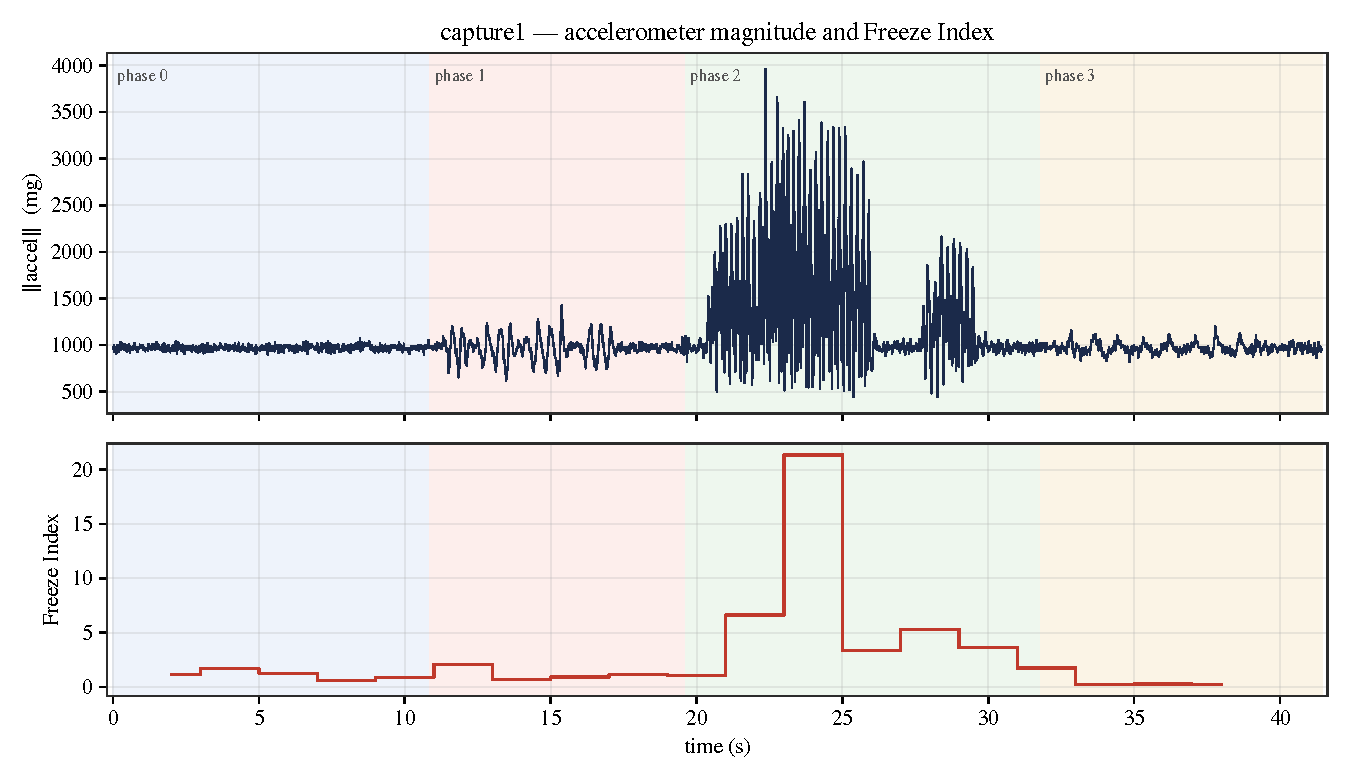
\includegraphics[width=0.92\linewidth]{capture1_trace.pdf}
\caption{Capture~1 --- accelerometer magnitude (top) and Freeze Index (bottom) with
protocol phases shaded. The FI spikes only in phase~2 (freeze).}
\label{fig:cap1}
\end{figure}

\begin{table}[H]
\centering
\caption{Per-phase Freeze Index, capture~1 (4\,s windows, 2\,s hop).}
\begin{tabular}{@{}c l c c c c@{}}
\toprule
\textbf{Phase} & \textbf{Activity} & \textbf{$n$ win.} & \textbf{FI mean} & \textbf{FI median} & \textbf{FI max}\\
\midrule
0 & still           & 5 & 1.13 & 1.15 & 1.71\\
1 & walk            & 4 & 1.20 & 1.03 & 2.08\\
2 & \textbf{freeze} & 6 & \textbf{6.89} & \textbf{4.45} & \textbf{21.35}\\
3 & walk            & 4 & 0.63 & 0.26 & 1.74\\
\bottomrule
\end{tabular}
\end{table}

\begin{figure}[H]
\centering
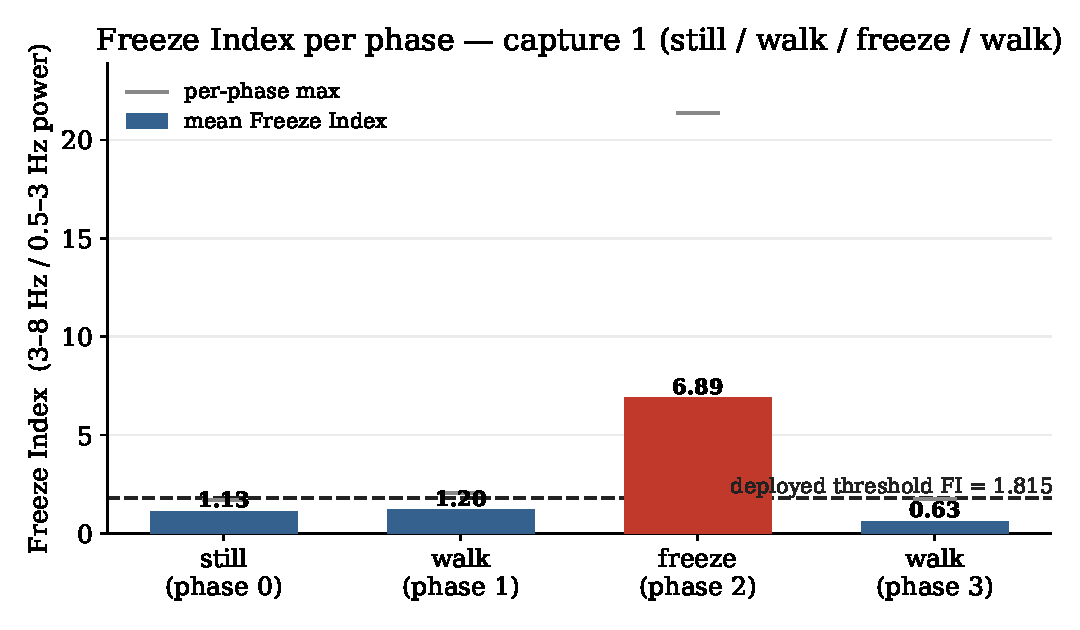
\includegraphics[width=0.82\linewidth]{fi_per_phase.pdf}
\caption{Mean Freeze Index per phase (capture~1) with the deployed decision
threshold. The freeze phase sits far above every walking/standing phase; the grey
ticks mark each phase's maximum.}
\label{fig:bar}
\end{figure}

\subsection{Defining ``accuracy'': the confusion matrix}
Every \SI{2}{\second} decision is scored against its protocol label as one of four
outcomes (Table~\ref{tab:cm2x2}). Writing $TP,FP,TN,FN$ for the counts, the metrics
this worksheet uses are
\[
\mathrm{sensitivity}=\frac{TP}{TP+FN},\qquad
\mathrm{specificity}=\frac{TN}{TN+FP},
\]
\[
\mathrm{precision}=\frac{TP}{TP+FP},\qquad
\mathrm{accuracy}=\frac{TP+TN}{TP+FP+TN+FN}.
\]

\begin{table}[H]
\centering
\caption{The $2\times2$ confusion matrix. Columns are what the detector decides; rows
are the ground truth from the protocol phase.}
\label{tab:cm2x2}
\small
\begin{tabular}{@{}l c c@{}}
\toprule
 & \textbf{Detector: freeze} & \textbf{Detector: no-freeze}\\
\midrule
\textbf{Truly freeze}    & TP \emph{(hit)}         & FN \emph{(missed freeze)}\\
\textbf{Truly no-freeze} & FP \emph{(false alarm)} & TN \emph{(correct clear)}\\
\bottomrule
\end{tabular}
\end{table}

\textbf{Why not a single ``accuracy'' number.} Take the subject-independent CNN
(Fig.~\ref{fig:cm}, $n=\num{8982}$ windows): $TN=\num{6842}$, $FP=\num{1285}$,
$FN=248$, $TP=607$, giving
\[
\mathrm{sens}=\tfrac{607}{855}=0.71,\qquad
\mathrm{spec}=\tfrac{6842}{8127}=0.84,\qquad
\mathrm{prec}=\tfrac{607}{1892}=0.32,\qquad
\mathrm{acc}=\tfrac{7449}{8982}=0.83.
\]
The accuracy of 0.83 looks strong, but it is carried almost entirely by the \num{6842}
easy true negatives. It hides that nearly a third of freezes are \emph{missed}
(sensitivity 0.71) and that only a third of freeze flags are \emph{correct} (precision
0.32) --- precisely the two failures a monitor is judged on. That is why the headline
is sensitivity and specificity, not accuracy.

\subsection{Choosing the threshold: a sensitivity/specificity sweep}
The deployed cut-off is measured, not guessed. We swept the Freeze-Index threshold on
capture~1, scoring all 19 windows against their phase label (6 freeze, 13 non-freeze).
Table~\ref{tab:sweep} gives the confusion counts and metrics at each threshold, with
Youden's $J=\mathrm{sens}+\mathrm{spec}-1$ as a single balanced score.

\begin{table}[H]
\centering
\caption{Freeze-Index threshold sweep on capture~1 (19 windows; 6 freeze, 13
non-freeze). $J$ is maximised on the plateau from $\mathrm{FI}=2.10$ upward; the board
deploys $1.815$ (bold rows).}
\label{tab:sweep}
\small
\begin{tabular}{@{}c c c c c c c c c@{}}
\toprule
\textbf{FI thr} & \textbf{TP} & \textbf{FP} & \textbf{TN} & \textbf{FN}
 & \textbf{sens} & \textbf{spec} & \textbf{acc} & \textbf{Youden $J$}\\
\midrule
1.00          & 6 & 6 & 7  & 0 & 1.00 & 0.54 & 0.68 & 0.54\\
1.50          & 5 & 3 & 10 & 1 & 0.83 & 0.77 & 0.79 & 0.60\\
\textbf{1.815}& 5 & 1 & 12 & 1 & 0.83 & 0.92 & 0.89 & 0.76\\
\textbf{2.10} & 5 & 0 & 13 & 1 & 0.83 & 1.00 & 0.95 & \textbf{0.83}\\
3.00          & 5 & 0 & 13 & 1 & 0.83 & 1.00 & 0.95 & 0.83\\
4.00          & 3 & 0 & 13 & 3 & 0.50 & 1.00 & 0.84 & 0.50\\
\bottomrule
\end{tabular}
\end{table}

Two things stand out. \textbf{(i)~Accuracy is a misleading objective.} At
$\mathrm{FI}>4.0$ the accuracy is still 0.84 --- as high as anywhere sensible --- yet
sensitivity has collapsed to 0.50: half the freezes are missed. Optimising accuracy
would push the threshold the \emph{wrong} way, whereas Youden's $J$ (and the
sensitivity/specificity pair) does not have this failure. \textbf{(ii)~The deployed
$\mathrm{FI}=1.815$ trades a little specificity for sensitivity.} The analysis optimum
on this clean capture is the $2.10$ plateau (sens 0.83, spec 1.00), but the board
ships the lower $1.815$ (sens 0.83, spec 0.92 here) so it stays sensitive on harder
sessions, leaning on the movement-energy gate and debounce (Task~4) to suppress the
single extra false positive this admits.

\subsection{A noisier session: where confounds bite}
Figure~\ref{fig:smoke} shows the longer ``smoketest'' session (44 windows, 10 freeze).
The freeze separation is still visible (freeze-phase FI median 3.49), but on this
noisier capture several confound windows cross the threshold. At
$\mathrm{FI}>1.70$, 8 of the 10 freezes are caught (sensitivity 0.80) while 8 of the
34 non-freeze windows also fire (specificity 0.76) --- the worst reaching FI~10.23 in
vigorous walking and FI~3.40 in quiet standing. These false positives, absent on the
clean capture, are exactly what the movement-energy gate and debounce in Task~4 are
built to remove.

\begin{figure}[H]
\centering

\includegraphics[width=0.92\linewidth]{smoketest_trace.pdf}
\caption{Smoketest (\SI{91}{\second}) --- a longer, noisier session. The Freeze-Index
axis is capped at 12 so the confound transients are visible: several walking and
standing windows briefly cross the $\mathrm{FI}=1.70$ operating line (worst: walk
$10.23$, stand $3.40$), while the genuine freeze (phase~2) runs far off-scale
(peak~$\approx 806$). This separation is what makes the gate and debounce effective.}
\label{fig:smoke}
\end{figure}

% ====================================================================
\section{Task 4 --- Limitations of the prototype}
\label{sec:task4}

\subsection{What features are present in the positive (freeze) readings?}
A sustained burst of \SIrange{3}{8}{\hertz} oscillation on the accelerometer
magnitude, \emph{together with} the collapse of the \SIrange{0.5}{3}{\hertz} stepping
rhythm. Numerically this is a large Freeze Index: capture~1 freeze FI mean 6.89 vs
walk 1.20 and still 1.13 (Fig.~\ref{fig:bar}); smoketest freeze FI median 3.49. The
freeze band also carries high tremor power.

\subsection{How are these features detected in code?}
On the board, two cascaded second-order band-pass filters compute the freeze-band
and locomotor-band power of each window; their ratio is the Freeze Index
(\texttt{computeFI()}, Listing~\ref{lst:detect}). A window is declared a freeze only
if FI exceeds the threshold \emph{and} the movement-energy gate passes. The identical
ratio is computed offline with a Welch PSD (Appendix~\ref{app:dsp}) for scoring.

\subsection{Is there unwanted overlap that causes false positives?}
Yes. Vigorous walking transients and hand-handling of the board put transient energy
into the freeze band, momentarily raising FI. Concretely, in the smoketest a standing
window reached FI~3.40 and a walking window reached FI~10.23 --- both well above the
$\mathrm{FI}=1.70$ operating point, so both are false positives. This is exactly why
specificity falls from 100\,\% on the clean capture (FI$>$2.10) to 76\,\% on the
noisier one (FI$>$1.70).

\subsection{How are false positives reduced in this first prototype (within a week)?}
Three mitigations, all implemented on-device (Listing~\ref{lst:detect}):
\begin{enumerate}[leftmargin=1.6em]
\item \textbf{Movement-energy gate.} Because FI is a ratio, quiet standing can make it
      explode from noise alone. We require the summed band power
      $(P_f+P_l)$ to exceed a floor before any freeze is accepted; below the floor the
      state is forced to \texttt{STILL}. The floor is \emph{calibrated per wearer}
      (4$\times$ resting energy, clamped to \numrange{8}{20}).
\item \textbf{Two-window debounce.} A freeze must persist for
      \texttt{CONFIRM\_ON}~$=2$ consecutive \SI{2}{\second} windows before it is
      confirmed, and clears after \texttt{CONFIRM\_OFF}~$=2$ clear windows. Isolated
      single-window spikes (the smoketest false positives above) are rejected.
\item \textbf{Per-wearer calibration.} Button-A measures the resting floor at boot, so
      the gate adapts to the individual rather than using a fixed constant.
\end{enumerate}

\subsection{Better ways to reduce false positives, given more time}
Replace the hand-tuned threshold with a \emph{learned} model trained across many
people. We trained a small convolutional network on the public \textbf{Daphnet} FoG
benchmark and evaluated it \textbf{subject-independently} (Leave-One-Subject-Out:
train on all but one patient, test on the held-out patient, repeat). Pooled over
\num{8982} test windows the CNN scores \textbf{sensitivity 71\,\% and specificity
84\,\%} (Fig.~\ref{fig:cm}), and it holds up --- with spread --- across individual
held-out patients (Fig.~\ref{fig:persub}). A complementary \emph{interpretable} model
(a random forest) lets us sweep the whole operating curve and expose the
low-prevalence trade-off; that fuller benchmark evaluation, with the ROC, the
precision--recall curve and the positive-predictive-value calculation, is in
Appendix~\ref{app:eval}.

\begin{keybox}
\textbf{Honest reading of the numbers.} The CNN's 71\,/\,84 is \emph{lower} than the
prototype's single-session 83\,/\,100. That is the point: the single clean session
\emph{overstates} real-world accuracy, because the detector is tuned to one person on
one day. The subject-independent figure is the trustworthy estimate, and the gap
between them is the generalisation challenge a deployed device must close --- with
more data, per-wearer personalisation, and richer features.
\end{keybox}

\begin{figure}[H]
\centering
\begin{minipage}[t]{0.49\linewidth}
\centering
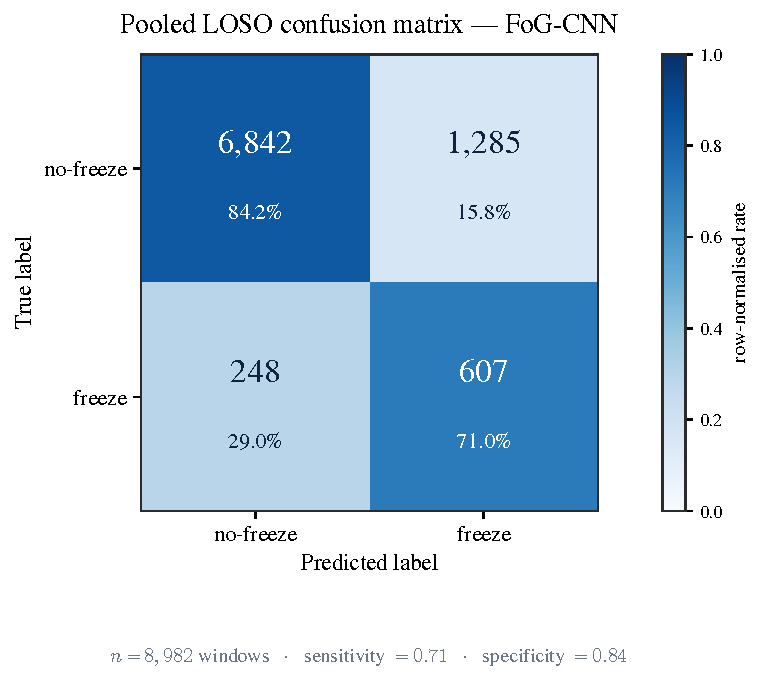
\includegraphics[width=\linewidth]{confusion_matrix.pdf}
\caption{CNN, subject-independent (LOSO) on Daphnet --- pooled confusion matrix:
sensitivity 0.71, specificity 0.84, $n=8{,}982$ windows.}
\label{fig:cm}
\end{minipage}\hfill
\begin{minipage}[t]{0.49\linewidth}
\centering
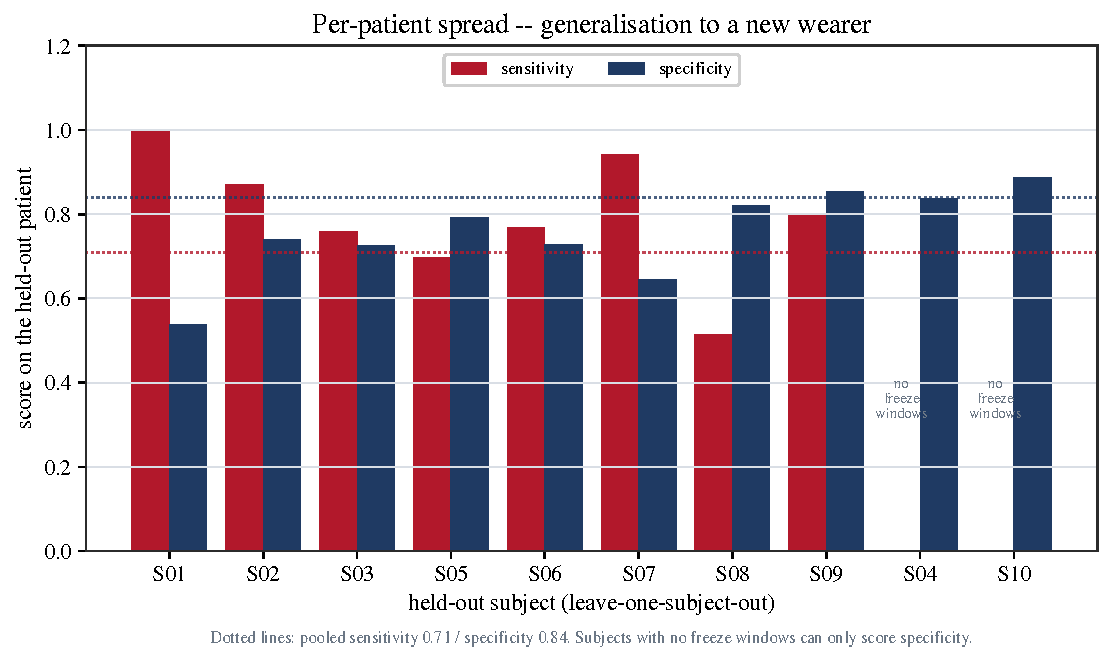
\includegraphics[width=\linewidth]{per_subject.pdf}
\caption{The same CNN, broken down per held-out patient. Sensitivity varies between
individuals; two subjects (S04, S10) contributed no freeze episodes.}
\label{fig:persub}
\end{minipage}
\end{figure}

\subsection{Are false negatives likely? How are they mitigated?}
Yes --- this is the more dangerous error for a monitor. An \emph{akinetic} freeze that
presents as a near-complete stop, with little trembling, has low power in
\emph{both} bands: FI stays low and the movement gate may even read it as
``standing''. We observed exactly this in the \texttt{ankle\_run} session
(Fig.~\ref{fig:ankle}), where the freezes were performed as standing pauses rather
than trembling-in-place: freeze-phase FI fell to 0.55 and 0.34 --- \emph{below}
walking --- and threshold scoring collapsed to 5\,\% sensitivity. Mitigations:
\begin{itemize}
\item \textbf{Detect by absence of gait.} Add features that flag the sudden loss of
      the expected \SIrange{0.5}{3}{\hertz} stepping rhythm after walking, so an
      akinetic freeze is caught by what \emph{stops} rather than what trembles.
\item \textbf{Stride-time variability / cadence breakdown} as a complementary feature.
\item \textbf{Lower the threshold} to raise sensitivity, explicitly trading away
      specificity --- the operating point can be chosen along the ROC
      (Fig.~\ref{fig:roc}) to suit a clinician's preference.
\item \textbf{Wearer coaching}, since freeze presentation varies between patients.
\end{itemize}

\begin{figure}[H]
\centering
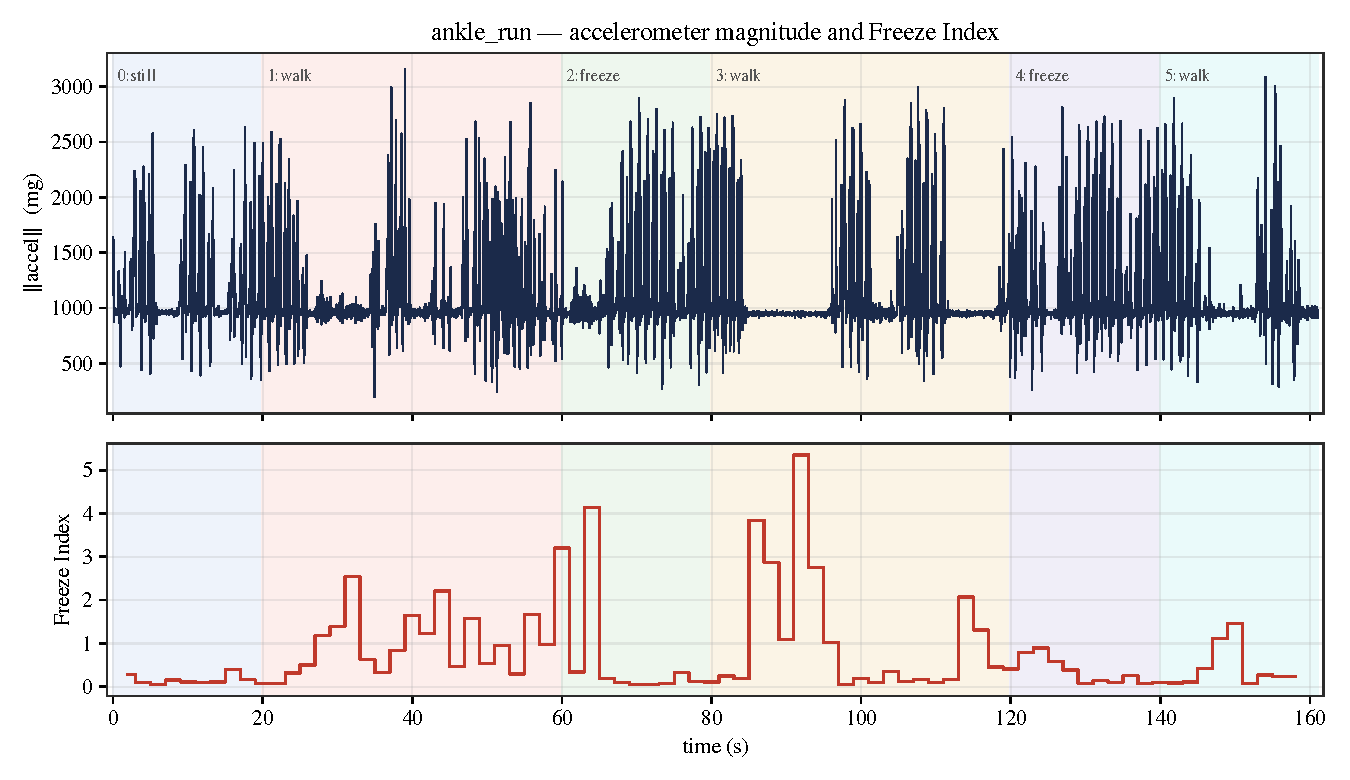
\includegraphics[width=0.92\linewidth]{ankle_run_trace.pdf}
\caption{\texttt{ankle\_run} --- a false-negative case. The large accelerometer
bursts fall in the \emph{walk} phases; the Freeze Index stays low through both
``freeze'' phases (2 and 4), which were performed as standing pauses. The detector
correctly cannot see a freeze that was not produced as a trembling-in-place event.}
\label{fig:ankle}
\end{figure}

\subsection{Summary: an error taxonomy}
Table~\ref{tab:errtax} consolidates the prototype's failure modes, the real evidence
for each, how it is handled within this one-week build, and what is left for future
work.

\begin{table}[H]
\centering
\caption{Error taxonomy for the on-board detector. ``Status'' is the state in this
one-week prototype; FP $=$ false positive, FN $=$ false negative.}
\label{tab:errtax}
\footnotesize
\renewcommand{\arraystretch}{1.35}
\begin{tabular}{@{}>{\raggedright\arraybackslash}p{2.2cm} >{\raggedright\arraybackslash}p{3.5cm} >{\raggedright\arraybackslash}p{2.6cm} >{\raggedright\arraybackslash}p{3.5cm} >{\raggedright\arraybackslash}p{1.9cm}@{}}
\toprule
\textbf{Error} & \textbf{Mechanism} & \textbf{Evidence} & \textbf{Mitigation} & \textbf{Status}\\
\midrule
FP --- quiet standing & FI is a ratio: sensor-noise over sensor-noise can be large & gate rejects sub-floor energy & movement-energy gate $(P_f{+}P_l>\text{floor})$ & resolved\\
FP --- walking transient & vigorous steps leak energy into the 3--8\,Hz band & smoketest walk window FI~10.23 & two-window debounce (\texttt{CONFIRM\_ON}=2) & mostly resolved\\
FP --- device handling & touching/adjusting the board adds broadband energy & --- & gate $+$ debounce; secure mounting & mostly resolved\\
FN --- akinetic freeze & near-complete stop: low power in \emph{both} bands & ankle\_run freeze FI 0.55, 0.34 & absence-of-gait feature; lower threshold & open (future)\\
FN --- very short freeze & briefer than the two-window confirm time & --- & shorten hop or \texttt{CONFIRM\_ON} (costs FP) & trade-off\\
\bottomrule
\end{tabular}
\end{table}

% ====================================================================
\section{Task 5 --- Final code}
\label{sec:task5}

Listing~\ref{lst:detect} is the deployed on-board detector. The mitigations from
Task~4 are highlighted in the comments: the \textbf{threshold} \texttt{FI\_THRESHOLD
= 1.815}, the \textbf{movement-energy gate} \texttt{last\_energy > still\_floor}, and
the \textbf{two-window debounce} via \texttt{on\_count} / \texttt{off\_count}. The
floor \texttt{still\_floor} is set by per-wearer calibration (clamped \numrange{8}{20}).

\begin{lstlisting}[style=cpp,label={lst:detect},emph={FI_THRESHOLD,still_floor,STILL_MARGIN,CONFIRM_ON,CONFIRM_OFF,on_count,off_count},emphstyle={\color{brick}\bfseries},caption={On-board freeze detector (Circuit Playground, cpx\_fog\_standalone.ino). The \textbf{threshold} and gate parameters fixed in Task~3 and the three Task~4 false-positive mitigations are \textcolor{brick}{\textbf{emphasised in red}} and flagged in the inline comments: the movement-energy \textbf{gate} (\texttt{still\_floor}), the \textbf{threshold} test (\texttt{FI\_THRESHOLD}), and the two-window \textbf{debounce} (\texttt{on\_count}/\texttt{off\_count}).}]
const float   FI_THRESHOLD = 1.815f;   // freeze threshold (Task 3 sweep)
float         still_floor   = 12.0f;   // movement-energy gate, per-wearer (8..20)
const float   STILL_MARGIN  = 4.0f;    // floor = 4 x resting band-power
const uint8_t CONFIRM_ON    = 2;       // need 2 consecutive freeze windows
const uint8_t CONFIRM_OFF   = 2;       // need 2 consecutive clear windows

float computeFI() {                    // 4 s window -> Freeze Index
  static float w[WINDOW];
  float mean = 0.0f;
  for (uint16_t i = 0; i < WINDOW; i++) { w[i] = ring[(head + i) % WINDOW]; mean += w[i]; }
  mean /= WINDOW;
  for (uint16_t i = 0; i < WINDOW; i++) w[i] -= mean;     // remove gravity/DC
  g_pf = runBand(FREEZE_SOS, w, WINDOW);   // 3-8 Hz band power  (biquad cascade)
  g_pl = runBand(LOCO_SOS,   w, WINDOW);   // 0.5-3 Hz band power
  return g_pf / (g_pl + 1e-9f);            // Eq. (1): the Freeze Index
}

// --- every HOP (2 s): the gated, debounced decision -----------------
last_fi     = computeFI();
last_energy = g_pf + g_pl;                       // movement energy (both bands)

bool moving = last_energy > still_floor;         // GATE: reject quiet standing
bool freeze = moving && (last_fi > FI_THRESHOLD);// THRESHOLD on a moving wearer
g_state     = !moving ? STILL : (freeze ? FREEZE : WALKING);

if (freeze) { on_count++;  off_count = 0; }      // DEBOUNCE: count run length
else        { off_count++; on_count  = 0; }
if (!cueing && on_count  >= CONFIRM_ON)  { cueing = true;  freezeEpisodes++; }
else if (cueing && off_count >= CONFIRM_OFF){ cueing = false; }   // confirmed clear
\end{lstlisting}

The band-pass coefficients, the biquad cascade and the per-wearer calibration routine
that produces \texttt{still\_floor} are listed in Appendix~\ref{app:filters}. The
offline scoring uses the identical mathematics in Python (Appendix~\ref{app:dsp}); the
two implementations were cross-checked so that the worksheet numbers and the on-body
behaviour agree.

% ====================================================================
\appendix
\section{Worked protocol example (provided with brief)}
\label{app:protocol}

A structured 20-minute protocol for evaluating walking detection against confounds,
adapted to the ankle FoG task:

\begin{table}[H]
\centering
\begin{tabular}{@{}c l c@{}}
\toprule
\textbf{Phase} & \textbf{Activity} & \textbf{Duration}\\
\midrule
1 & Baseline (stand / sit still)            & \SI{2}{\minute}\\
2 & Normal walking                          & \SI{4}{\minute}\\
3 & Fast walking                            & \SI{2}{\minute}\\
4 & Confounds: arm-swing, shaking, sitting tasks, weight-shift & \SI{8}{\minute}\\
5 & Mixed real-world (walk, stop, turn, pick up, sit-stand)    & \SI{4}{\minute}\\
\bottomrule
\end{tabular}
\end{table}

\noindent Key confounders to watch: arm-swinging while stationary, device handling,
external vibration, and slow weight-shifting --- each can mimic part of the gait
signature and is a candidate false-positive source.

% --------------------------------------------------------------------
\section{Data-logging firmware (excerpt)}
\label{app:logger}

The store-and-forward logger writes one 7-byte record per sample at \SI{64}{\hertz}
with an auto-incrementing phase label. NeoPixel colours guide the untethered wearer
(cyan = still, green = walk, red = freeze).

\begin{lstlisting}[style=cpp,caption={Scripted schedule and per-sample logging (cpx\_fog\_logger.ino).}]
const Phase SCHED[] = {                 // segment index = the logged phase column
  { "STILL",  20, false },  // 0
  { "WALK",   40, false },  // 1
  { "FREEZE", 20, true  },  // 2
  { "WALK",   40, false },  // 3
  { "FREEZE", 20, true  },  // 4   ... cycle repeats, ends on a STILL block
};

// steady 64 Hz sampling inside the RUNNING state:
float ax = CircuitPlayground.motionX();           // m/s^2
float ay = CircuitPlayground.motionY();
float az = CircuitPlayground.motionZ();
pushRecord((int16_t)(ax * MS2_TO_MG),             // store as int16 milli-g
           (int16_t)(ay * MS2_TO_MG),
           (int16_t)(az * MS2_TO_MG), segIdx);    // + the phase label
\end{lstlisting}

% --------------------------------------------------------------------
\section{On-board band-pass filters and calibration}
\label{app:filters}

The Freeze Index needs the power in two frequency bands. On the board each band is a
second-order Butterworth band-pass realised as two cascaded second-order sections
(coefficients exported from the offline design at \SI{64}{\hertz}) and applied as a
Direct-Form-II-transposed biquad cascade. \texttt{runBand()} returns
$\sum y^2$ over the window, which is proportional to band power; the proportionality
constant cancels in the FI ratio (Eq.~\ref{eq:fi}).

\begin{lstlisting}[style=cpp,caption={Deployed band-pass coefficients and the biquad cascade (cpx\_fog\_standalone.ino).}]
struct Sos { float b0, b1, b2, a1, a2; };    // a0 normalised to 1
const uint8_t N_SOS = 2;                      // order-2 Butterworth -> 2 sections

const Sos FREEZE_SOS[N_SOS] = {               // 3-8 Hz freeze band
  { 0.04427971f,  0.08855942f, 0.04427971f, -1.24067070f, 0.62897179f },
  { 1.00000000f, -2.00000000f, 1.00000000f, -1.69751871f, 0.79495806f },
};
const Sos LOCO_SOS[N_SOS] = {                 // 0.5-3 Hz locomotor band
  { 0.01278734f,  0.02557469f, 0.01278734f, -1.69059402f, 0.75072617f },
  { 1.00000000f, -2.00000000f, 1.00000000f, -1.93848688f, 0.94143123f },
};

// Run one band through the cascade; return sum(y^2) over the window (= band power).
float runBand(const Sos *sos, const float *x, uint16_t n) {
  float z1[N_SOS] = {0}, z2[N_SOS] = {0}, sumsq = 0.0f;
  for (uint16_t i = 0; i < n; i++) {
    float in = x[i];
    for (uint8_t s = 0; s < N_SOS; s++) {              // direct-form-II transposed
      float out = sos[s].b0 * in + z1[s];
      z1[s] = sos[s].b1 * in - sos[s].a1 * out + z2[s];
      z2[s] = sos[s].b2 * in - sos[s].a2 * out;
      in = out;
    }
    sumsq += in * in;
  }
  return sumsq;                               // proportionality cancels in FI ratio
}
\end{lstlisting}

\textbf{Per-wearer calibration of the gate.} Pressing button~A while standing still
measures the resting band-power over one window and sets the movement-energy floor to
\texttt{STILL\_MARGIN}~$\times$~resting, clamped to \numrange{8}{20}. The clamp band
comes from bench measurement: a dead-still board on this hardware reads energy
$\approx 2.5$ (up to $\sim$5 with handling transients) while \emph{any} deliberate
motion drives it into the tens-to-hundreds, so any floor in \numrange{8}{20} sits
safely above still-noise yet well below real gait.

\begin{lstlisting}[style=cpp,caption={Button-A calibration of the movement-energy floor (cpx\_fog\_standalone.ino).}]
const float STILL_MARGIN = 4.0f;   // floor = margin x resting energy
const float MIN_FLOOR    = 8.0f;   // stay ABOVE measured still-noise (~5)
const float MAX_FLOOR    = 20.0f;  // ... yet well BELOW real-motion energy (tens+)

if (calib_left == 0 && filled >= WINDOW) {
  computeFI();                          // fills g_pf, g_pl for the still window
  float rest  = g_pf + g_pl;           // resting movement energy (both bands)
  still_floor = STILL_MARGIN * rest;   // gate threshold for THIS wearer + board
  if (still_floor < MIN_FLOOR) still_floor = MIN_FLOOR;
  if (still_floor > MAX_FLOOR) still_floor = MAX_FLOOR;
}
\end{lstlisting}

% --------------------------------------------------------------------
\section{Offline analysis code (excerpt)}
\label{app:dsp}

The Python reference implementation (\texttt{fog/dsp.py}) that scores the captures.
It is the same Freeze Index and movement-energy used on the board, validated against
the firmware output.

\begin{lstlisting}[style=py,caption={Freeze Index and movement-energy (fog/dsp.py).}]
def magnitude(window):                         # (T,3) accel -> (T,) mean-removed |a|
    mag = np.linalg.norm(window, axis=1)
    return mag - mag.mean()                    # strip gravity / DC

def band_power(sig1d, fs, band):               # power in [lo,hi) Hz via Welch PSD
    f, pxx = signal.welch(sig1d, fs=fs, nperseg=min(len(sig1d), 256))
    lo, hi = band
    mask = (f >= lo) & (f < hi)
    df = float(f[1] - f[0])
    return float(np.sum(pxx[mask]) * df)

def freeze_index(window, fs=64):               # Eq. (1): Moore et al. 2008
    mag  = magnitude(window)
    loco = band_power(mag, fs, (0.5, 3.0))     # locomotor band
    return band_power(mag, fs, (3.0, 8.0)) / (loco + 1e-9)   # freeze / loco

def movement_energy(window, fs=64):            # gate signal: total band power
    mag = magnitude(window)
    return band_power(mag, fs, (0.5, 3.0)) + band_power(mag, fs, (3.0, 8.0))
\end{lstlisting}

\vspace{1em}
\begin{keybox}
\small\textbf{Reproducibility.} Every figure and number in this worksheet is produced
from the captures in \texttt{accuracy\_figs/captures/} by \texttt{analyze\_worksheet.py};
e.g.\ capture~1 is scored with\\
\texttt{\footnotesize python analyze\_worksheet.py accuracy\_figs/captures/capture1.csv -{}-freeze-phases 2}.
\end{keybox}

% --------------------------------------------------------------------
\section{Offline benchmark-model evaluation}
\label{app:eval}

To estimate how a \emph{learned} detector would generalise beyond our own captures, two
models were trained on the public \textbf{Daphnet} Freezing-of-Gait dataset
(B\"achlin \emph{et al.}, 2010) and evaluated \textbf{subject-independently} with
\emph{Leave-One-Subject-Out} (LOSO) cross-validation: train on every patient but one,
test on the held-out patient, and repeat so that every prediction is made on a wearer
the model never saw in training. Evaluating on the same person you trained on flatters
the result; LOSO is the honest estimate of field performance.

\textbf{Model 1 --- convolutional network (headline cross-subject estimate).} A small
1-D CNN over the windowed accelerometer signal. Pooling all held-out predictions
(\num{8982} windows) gives sensitivity 0.71 and specificity 0.84
(Fig.~\ref{fig:cm}); the per-patient breakdown (Fig.~\ref{fig:persub}) shows the
spread between individuals --- some patients freeze in ways the pooled model catches
easily, others much less so.

\textbf{Model 2 --- interpretable random forest (operating curve and prevalence).} A
random forest over hand-engineered band-power features. Because it emits a graded
score, every decision threshold can be swept to draw the full ROC (Fig.~\ref{fig:roc},
AUC~0.82) and precision--recall curve (Fig.~\ref{fig:pr}). The ROC lets a clinician
choose the sensitivity/specificity trade-off explicitly rather than accept one fixed
operating point.

\begin{figure}[H]
\centering
\begin{minipage}[t]{0.49\linewidth}
\centering
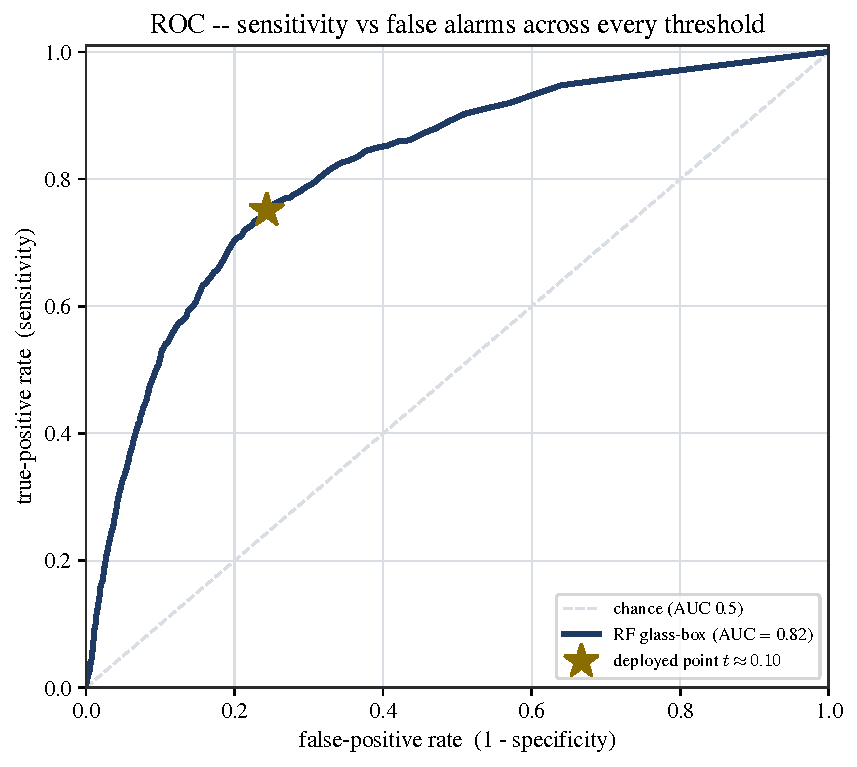
\includegraphics[width=\linewidth]{roc_curve.pdf}
\caption{ROC of the interpretable model across all thresholds (AUC~0.82). Each point
is a sensitivity/specificity trade-off a clinician could select.}
\label{fig:roc}
\end{minipage}\hfill
\begin{minipage}[t]{0.49\linewidth}
\centering
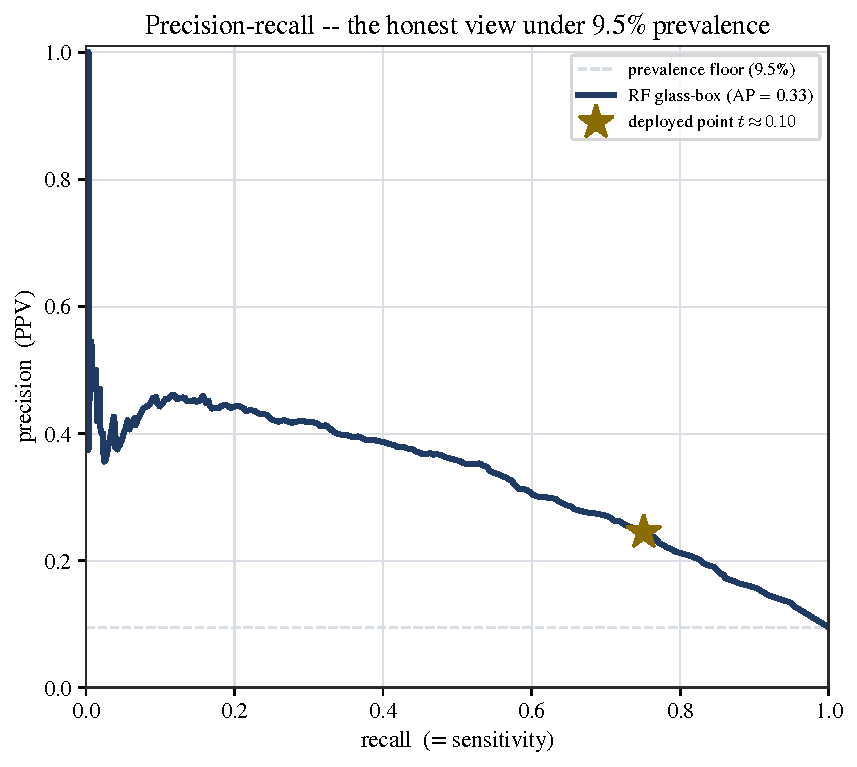
\includegraphics[width=\linewidth]{pr_curve.pdf}
\caption{Precision--recall for the same model. Average precision is 0.33 at the
dataset's 9.5\,\% freeze prevalence --- the realistic view.}
\label{fig:pr}
\end{minipage}
\end{figure}

\begin{keybox}
\textbf{Why precision matters more than ``accuracy'' here.} Freezes are only about
\textbf{9.5\,\%} of the Daphnet windows. At that prevalence even a good detector has
modest \emph{precision}. With sensitivity 0.71 and specificity 0.84 the positive
predictive value is
\[
\mathrm{PPV}=\frac{0.71\times0.095}{0.71\times0.095+(1-0.84)\times0.905}\approx 0.32,
\]
so only about a third of the windows flagged as a freeze are truly freezes --- and the
random forest's average precision (0.33) tells the same story. A bare ``accuracy''
figure would read $\sim$0.83 and hide this completely. This is exactly why the
worksheet reports sensitivity and specificity (and here precision/PPV) rather than
accuracy, and why Cadence is positioned as a \textbf{monitor} whose flags a clinician
reviews --- not an alarm that must be right every time.
\end{keybox}

% --------------------------------------------------------------------
\section*{References}
\addcontentsline{toc}{section}{References}
\begin{enumerate}[leftmargin=1.8em,label={[\arabic*]}]
\item S.\,T. Moore, H.\,G. MacDougall, W.\,G. Ondo. ``Ambulatory monitoring of
freezing of gait in Parkinson's disease.'' \emph{Journal of Neuroscience Methods},
167(2):340--348, 2008. \emph{(Defines the Freeze Index as the 3--8\,Hz $/$ 0.5--3\,Hz
accelerometer power ratio.)}
\item M. B\"achlin, M. Plotnik, D. Roggen, I. Maidan, J.\,M. Hausdorff, N. Giladi,
G. Tr\"oster. ``Wearable assistant for Parkinson's disease patients with the freezing
of gait symptom.'' \emph{IEEE Transactions on Information Technology in Biomedicine},
14(2):436--446, 2010. \emph{(Movement-energy gating; source of the Daphnet dataset.)}
\item Daphnet Freezing of Gait dataset, UCI Machine Learning Repository. Tri-axial
accelerometer recordings (ankle, thigh, trunk) from Parkinson's patients at
\SI{64}{\hertz}, with freeze annotations.
\end{enumerate}

\end{document}
